% begin module derivatives-as-function-ex1
\begin{frame}
\begin{example}[Example 1, p. 124]
The graph of a function $f$ appears below.  Use it to sketch the graph of the derivative $f'$.
\begin{columns}[c]
\column{.5\textwidth}
\ \only<handout:0| -3>{%
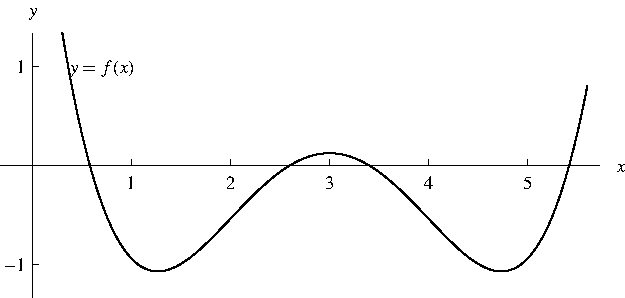
\includegraphics[height=2.9cm]{derivatives/pictures/03-02-ex1fa.pdf}%
}%
\only<handout:0| 4-5>{%
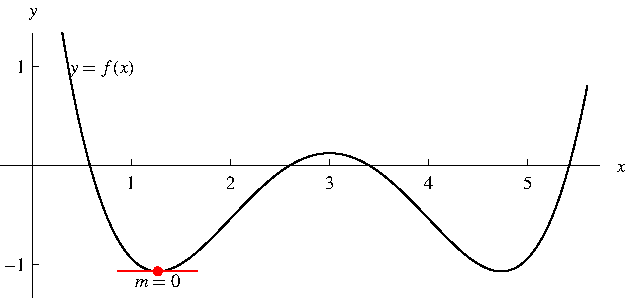
\includegraphics[height=2.9cm]{derivatives/pictures/03-02-ex1fb.pdf}%
}%
\only<handout:0| 6-7>{%
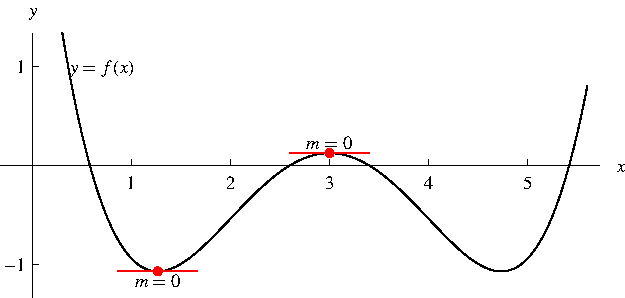
\includegraphics[height=2.9cm]{derivatives/pictures/03-02-ex1fc.pdf}%
}%
\only<handout:0| 8-10>{%
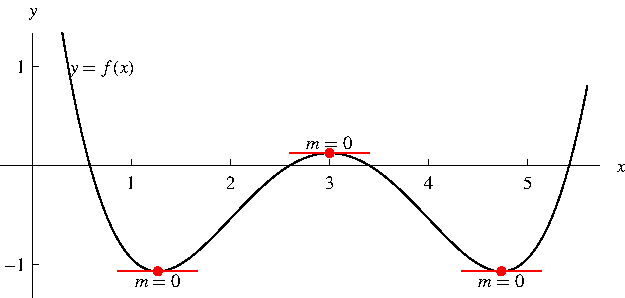
\includegraphics[height=2.9cm]{derivatives/pictures/03-02-ex1fd.pdf}%
}%
\only<handout:0| 11-13>{%
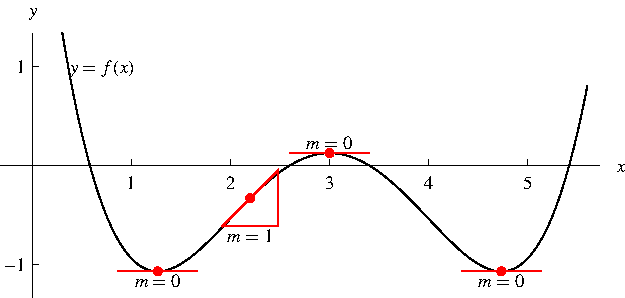
\includegraphics[height=2.9cm]{derivatives/pictures/03-02-ex1fe.pdf}%
}%
\only<14->{%
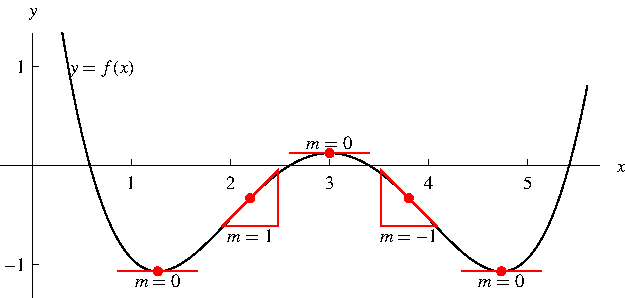
\includegraphics[height=2.9cm]{derivatives/pictures/03-02-ex1ff.pdf}%
}%

\ \only<handout:0| -4>{%
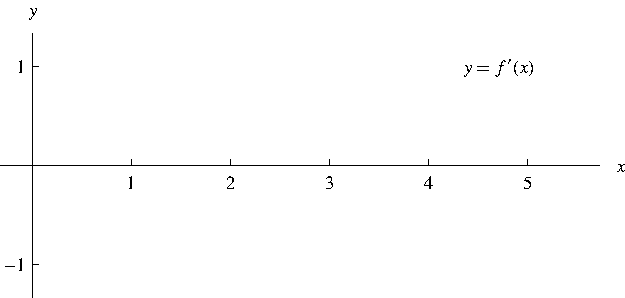
\includegraphics[height=2.9cm]{derivatives/pictures/03-02-ex1fprimea.pdf}%
}%
\only<handout:0| 5-6>{%
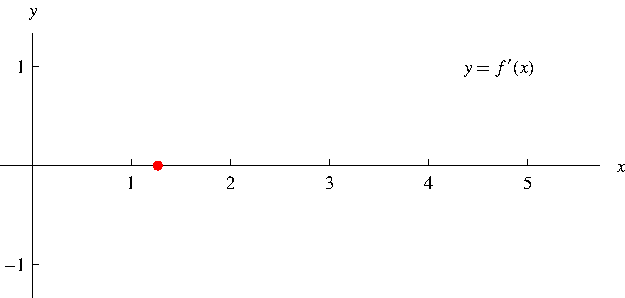
\includegraphics[height=2.9cm]{derivatives/pictures/03-02-ex1fprimeb.pdf}%
}%
\only<handout:0| 7-8>{%
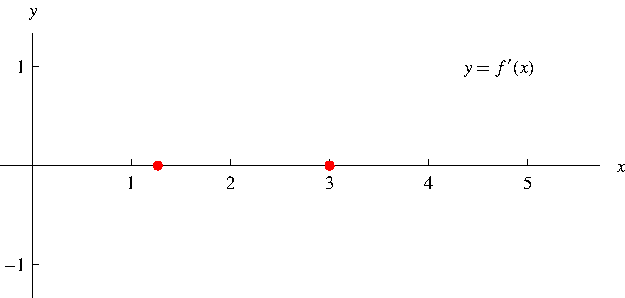
\includegraphics[height=2.9cm]{derivatives/pictures/03-02-ex1fprimec.pdf}%
}%
\only<handout:0| 9-11>{%
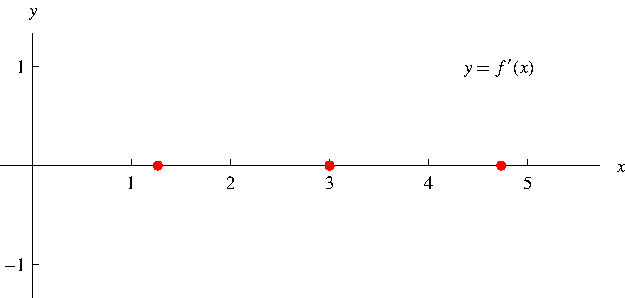
\includegraphics[height=2.9cm]{derivatives/pictures/03-02-ex1fprimed.pdf}%
}%
\only<handout:0| 12-14>{%
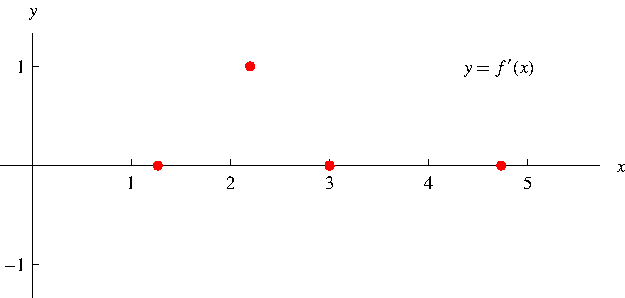
\includegraphics[height=2.9cm]{derivatives/pictures/03-02-ex1fprimee.pdf}%
}%
\only<handout:0| 15-17>{%
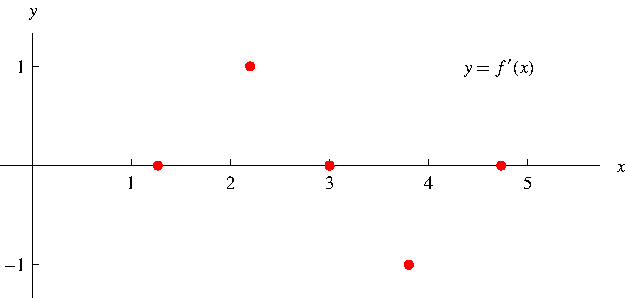
\includegraphics[height=2.9cm]{derivatives/pictures/03-02-ex1fprimef.pdf}%
}%
\only<18->{%
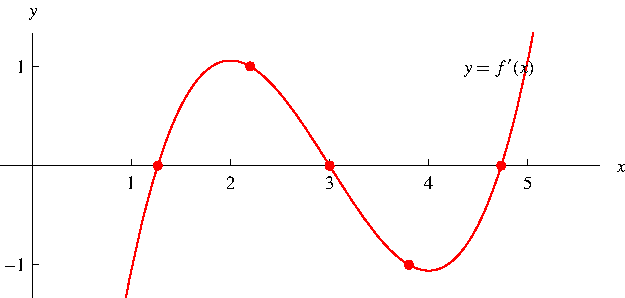
\includegraphics[height=2.9cm]{derivatives/pictures/03-02-ex1fprimeg.pdf}%
}%
\column{.5\textwidth}
\begin{itemize}
\item<2->  Find the points where the tangent is horizontal ($m = 0$).
\item<3->  That is where $f'$ is $0$.
\item<10->  Where the slope of the tangent to $f$ is $1$, $f'$ is $1$.
\item<13->  Where the slope of the tangent to $f$ is $-1$, $f'$ is $-1$.
\item<16->  Where the slope of the curve is negative, $f'$ is negative.
\item<17->  Where the slope of the curve is positive, $f'$ is positive.
\end{itemize}
\end{columns}
\end{example}
\end{frame}
% end module derivatives-as-function-ex1
